%% new commands
\newcommand{\mso}{MS 0735.6+7421}
\newcommand{\ms}{MS07}

%% load preferences
\documentclass[11pt]{article}
\usepackage{graphicx,common}
\usepackage[nonamebreak,numbers,sort&compress]{natbib}
\bibliographystyle{plainnat}
\setlength{\textwidth}{6.5in} 
\setlength{\textheight}{10in}
\setlength{\topmargin}{0in} 
\setlength{\oddsidemargin}{-0.13in}
\setlength{\evensidemargin}{0in} 
\setlength{\headheight}{-0.3in}
\setlength{\headsep}{0in} 
\setlength{\hoffset}{0in}
\setlength{\voffset}{0in}

%% get rid of blank line in bib
\let\oldbib=\thebibliography
\let\endoldbib=\endthebibliography
\renewenvironment{thebibliography}[1]{
  \begin{oldbib}{#1}
    \setlength{\parskip}{0pt}
    \setlength{\itemsep}{0pt}
}{\end{oldbib}}

%% start the doc
\begin{document}
\pagestyle{plain}
\pagenumbering{arabic}

\begin{center}
  {\bf\uppercase{MS 0735.6+7421: Observing The Most Powerful AGN
      Outburst at Low Radio Frequencies}}
\end{center}

\noindent{\bf{\uppercase{Scientific Justification}}}\\

Over the last decade, X-ray observations have revealed numerous
examples of complex interactions between relativistic outflows from
active galactic nuclei (AGN) and hot halos surrounding the host
galaxies \cite{hydraa0, perseus1}. Shocks and cavities resulting from
the AGN outflow-halo interaction provide a direct measure of the $pV$
work performed on the halo and thus are useful for estimating the
mechanical energy of an AGN outburst, \cite[see][for a
  review]{mcnamrev}. Using cavities as calorimeters, studies have
shown that AGN release $\sim 10^{55-62}$ erg of energy at rates of
$\sim 10^{41-46} ~\lum$, sufficient to offset the radiative losses of
the host halo \cite[\eg][]{birzan04, dunn06}. Further, in these
systems, short halo cooling times, the appearance of multiphase gas,
host galaxy star formation rates, and AGN activity are closely
correlated \cite{crawford99, edge01, haradent, rafferty06}, indicating
the presence of a cooling-heating feedback loop with AGN acting as
energy redistributors. These results have shaped prevailing galaxy
formation models such that they now utilize AGN feedback as the
primary means for regulating late-time galaxy evolution
\cite[\eg][]{croton06, bower06, sijacki07}. Though the understanding
of AGN feedback has improved greatly through the use of X-ray
observations, the details of how feedback energy is thermalized, how
AGN are fueled, and the fundamental properties of radio jets/lobes
remain elusive.

Of particular interest are extreme AGN outbursts ($E \ga 10^{61}$ erg)
in gas-poor hosts, such as Cygnus A, Hercules A, Hydra A, and
\mso\ (hereafter \ms) \cite{2006ApJ...644L...9W, herca, hydraa,
  ms0735}. In these systems the mass accretion processes which can
supply fuel to the SMBH are strained to the point of unrealistic
efficiencies. As a solution to this problem, it has been suggested
that these systems may be observational evidence that some AGN
outbursts are powered by the release of energy stored in a rapidly
rotating supermassive black hole (SMBH) \cite{msspin, minaspin}. The
extreme outburst energies may also drive the host cluster away from
hydrostatic equilibrium, induce bulk ICM motions, and distribute
metal-enriched gas far from the central galaxy
\cite{2007ApJ...660.1118G, hydrametal, 2009A&A...495..721S}. These
rare systems are thus important targets for studying the process of
AGN feedback, and in this proposal we focus on the most powerful AGN
outburst currently known, and the only one which has not been observed
at 74 MHz: \ms\ (energy $\sim 10^{62}$ erg; power $\sim 10^{45}
~\lum$). {\bf We propose to obtain a deep observation of \ms\ at 74
  MHz to complement already acquired GMRT radio data between 150--1400
  MHz and 500 ks of Chandra X-ray data to further study in-detail the
  properties of the radio jets/lobes and the energetics of the AGN
  outburst}.

Analysis of the cavities and large-scale shock in \ms\ using the X-ray
data alone provides good limits on the outburst energetics, gives
reasonable constraints on the age of radio lobes, but says little
about the jet/lobe compositions and radiative efficiencies. The
inclusion of broadband radio data addresses these disparities by
making it possible to take a complete census of the radiating particle
population. \ms\ is a steep-spectrum radio source, $\alpha > -2$, so
it is critical to our science objectives to obtain radio observations
at the lowest frequencies possible where the cavity system stores a
tremendous amount of energy in old radiating populations distributed
over large-scales. The 74 MHz data, in particular, is essential to the
study of \ms\ because it extends our knowledge of the radio spectrum
into the frequency regime where the break frequency is reliably
estimated.

By combining the total energy estimates from the X-ray analysis and
the synchrotron energy estimates from the radio analysis, the jet and
lobe magnetic field strengths, compositions, radiative efficiencies,
environmental pressure balance, degree of confinement, and deviation
from equipartition can be calculated and inferred
\cite[\eg][]{2003MNRAS.342..399G, 2004AJ....127...48L,
  2005MNRAS.364.1343D, 2006MNRAS.372.1741D, 2006ApJ...648..200D,
  birzan08, pjet}. We can also investigate secondary processes such as
matter entrainment and gas shocking by respectively mapping radio
source composition and comparing cavity dynamical ages with
synchrotron age estimates \cite[\eg][]{2006ApJ...644L...9W,
  birzan08}. In addition, the low-frequency radio emission (and most
definitely at 74 MHz) may reveal larger cavity volumes where higher
frequency emission has faded, thus providing better cavity volume
estimates and improved constraints on the \ms\ outburst energetics. In
these ways, the synergy between the X-ray and radio observations
provide vital information on the AGN outburst and an rare outlier in
the general process of AGN feedback.

\noindent{\bf{\uppercase{Technical Justification}}}\\

The EVLA is required to make the 74 MHz measurement requested because
it is the only radio observatory equipped with the instrumentation
capable of achieving the resolution and sensitivity to image the
diffuse, faint synchrotron structure of \ms. The observational
parameters needed to achieve our scientific goals were determined
using a 325 MHz VLA A-array image of \ms\ and the EVLA Exposure
Calculator\footnote{http://science.nrao.edu/evla/tools/exposure/exposurecalc.shtml}. At
74 MHz in A-array, assuming typical winter conditions and 25
operational antennas, a dual polarization, 1 sub-band setup with 2 MHz
of bandwidth and integration time of 10 hr will result in RMS noise
($1\sigma$; natural weighting) of $\approx 24$ mJy beam$^{-1}$. If 16
MHz of bandwidth is achieved, then the noise may be $\la 10$ mJy
beam$^{-1}$. Regardless, the predicted EVLA noise is much lower than
that of the 150 MHz GMRT observations which produced a high-fidelity
image. This suggests our requested observation will be sensitive to
faint emission features, reaching our goal of further investigating
the ICM-AGN interaction and radio source composition in this unique
cluster. The maximum half-power beam-widths will be $\approx 24\arcs$
with a time-smearing limited field-of-view (FOV) of $\approx 800\arcs$
(shown in Fig. \ref{fig:img}). For a \cosmo, the resolution equates to
84 kpc and the FOV $\approx 3$ Mpc, sufficient to resolve the radio
emission in the $\sim 200$ kpc across cavities and image the entire
radio source and cluster environment. Observing \ms\ during one 10 hr
session will sample a broad enough segment of the $uv$ plan to ensure
reliable imaging of the rich sub-GHz intensity structure.\\

\bibliography{cavagnolo}

%\small
%\noindent \input{short.bbl}
%\normalsize

%% \clearpage
%% {\def\section*#1{}
%%   \begin{thebibliography}{100}
%%   \bibitem{a} A et al. AA, 1:1--1, 2010.
%%   \end{thebibliography}
%% }

\clearpage
\begin{figure}[htp]
  \begin{center}
    \begin{minipage}{0.75\linewidth}
      \includegraphics[width=\textwidth]{ms07.ps}
    \end{minipage}
    \vspace{-2cm}
    \caption{Composite image of \ms\ showing the pair of $\sim 200
      kpc$ across cavities in the ICM. X-ray is in blue, optical is in
      yellow, and 325 MHz radio is in red. X-ray:
      NASA/CXC/Univ. Waterloo/B.McNamara; Optical:
      NASA/ESA/STScI/Univ. Waterloo/B.McNamara; Radio: NRAO/Ohio
      Univ./L.Birzan et al.}
    \label{fig:img}
  \end{center}
\end{figure}

\end{document}

% LocalWords:  andt
